\documentclass [a4paper] {report}
\usepackage{amsmath,amssymb,amsthm, bbm, graphicx,listings,braket,subfig,titlesec,cleveref,lipsum,mcode,xcolor-patch, textcomp,float,booktabs,siunitx, listings}
\usepackage[authoryear]{natbib}
\usepackage[section]{placeins}
\usepackage[margin=2.2cm]{geometry}
\titleformat{\chapter}{\normalfont\huge}{\thechapter.}{20pt}{\huge \bf}

\DeclareMathOperator*{\argmin}{arg\,min}
\DeclareMathOperator*{\argmax}{arg\,max}
\newcommand{\norm}[1]{\left\lVert #1 \right\rVert}

\begin{document}
	
	\begin{titlepage}
		\begin{center}
			
			\textsc{\LARGE IN4320 Machine Learning}\\[1.25cm]
			
			\rule{\linewidth}{0.5mm}\\[1.0cm]
			{\huge \bfseries Final Assignment }\\[0.6cm]
			\rule{\linewidth}{0.5mm}\\[1.5cm]
			
			\begin{minipage}{0.4\textwidth}
				\begin{flushleft} \large	
					\emph{Author:}\\
					\textsc{Milan Niestijl, 4311728}
				\end{flushleft}
			\end{minipage}
			
			\vfill
			{\large \today}
		\end{center}
	\end{titlepage}
	
	\section*{Introduction}
	In this assignment the task is to build a classifier that optimally predicts the test set of the "Human Activity Recognition" dataset, which is a six-class problem. Three of the classes correspond to highly active movements, whereas the other three correspond to relatively low activity. The available training ($X_{trn}$) and test ($X_{tst}$) set contain 5580 and 4719 instances, respectively, both having a 554-dimensional feature space. Lastly, it is known what subject the different training instances stem from, which may be used to improve the performance of the classifier somehow. In this report, it is discussed how the resulting classifier was obtained. Both the reasoning and the considerations that led to the final classifier are discussed. A final score on the test set of $0.97814$ was achieved. The estimated number of words in this document is 2430.\\
	

	\section*{Data analysis}
	It is important to get some understanding of the data. We therefore firstly use principal component analysis (PCA) to visualise the data. In figure \ref{singvals}, the singular values of the training data are shown. It can be seen that a large portion of the variance in the data is captured in the first few principal components, indicating that the data in the reduced space of the first three components is reasonably representative of the complete data. In figure \ref{Xtrn}, the resulting plot is shown. 
	
	\begin{figure}[H]
		\begin{center}
			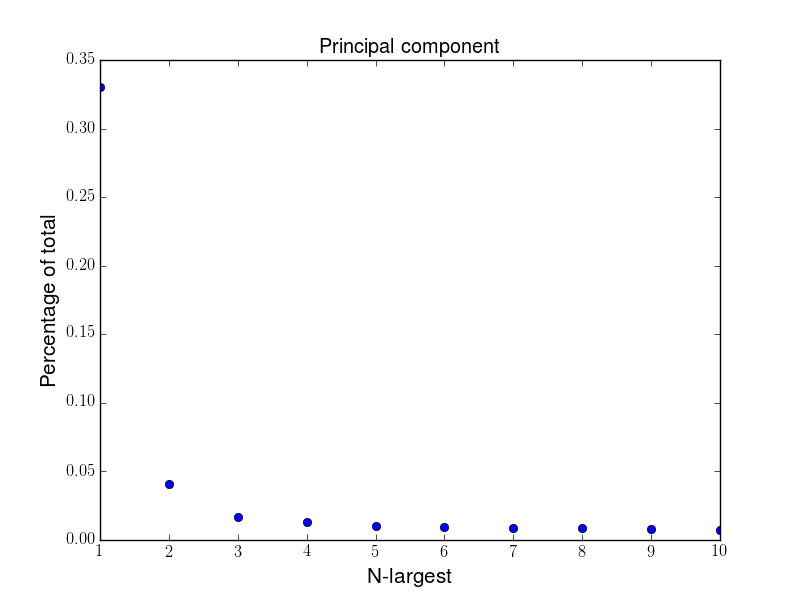
\includegraphics[scale=0.35]{Images/singvals.png}
		\end{center}
		\caption{Percentage of the variance coming from the first ten principal components.}
		\label{singvals}
	\end{figure}
	
	\begin{figure}[H]
		\begin{center}
			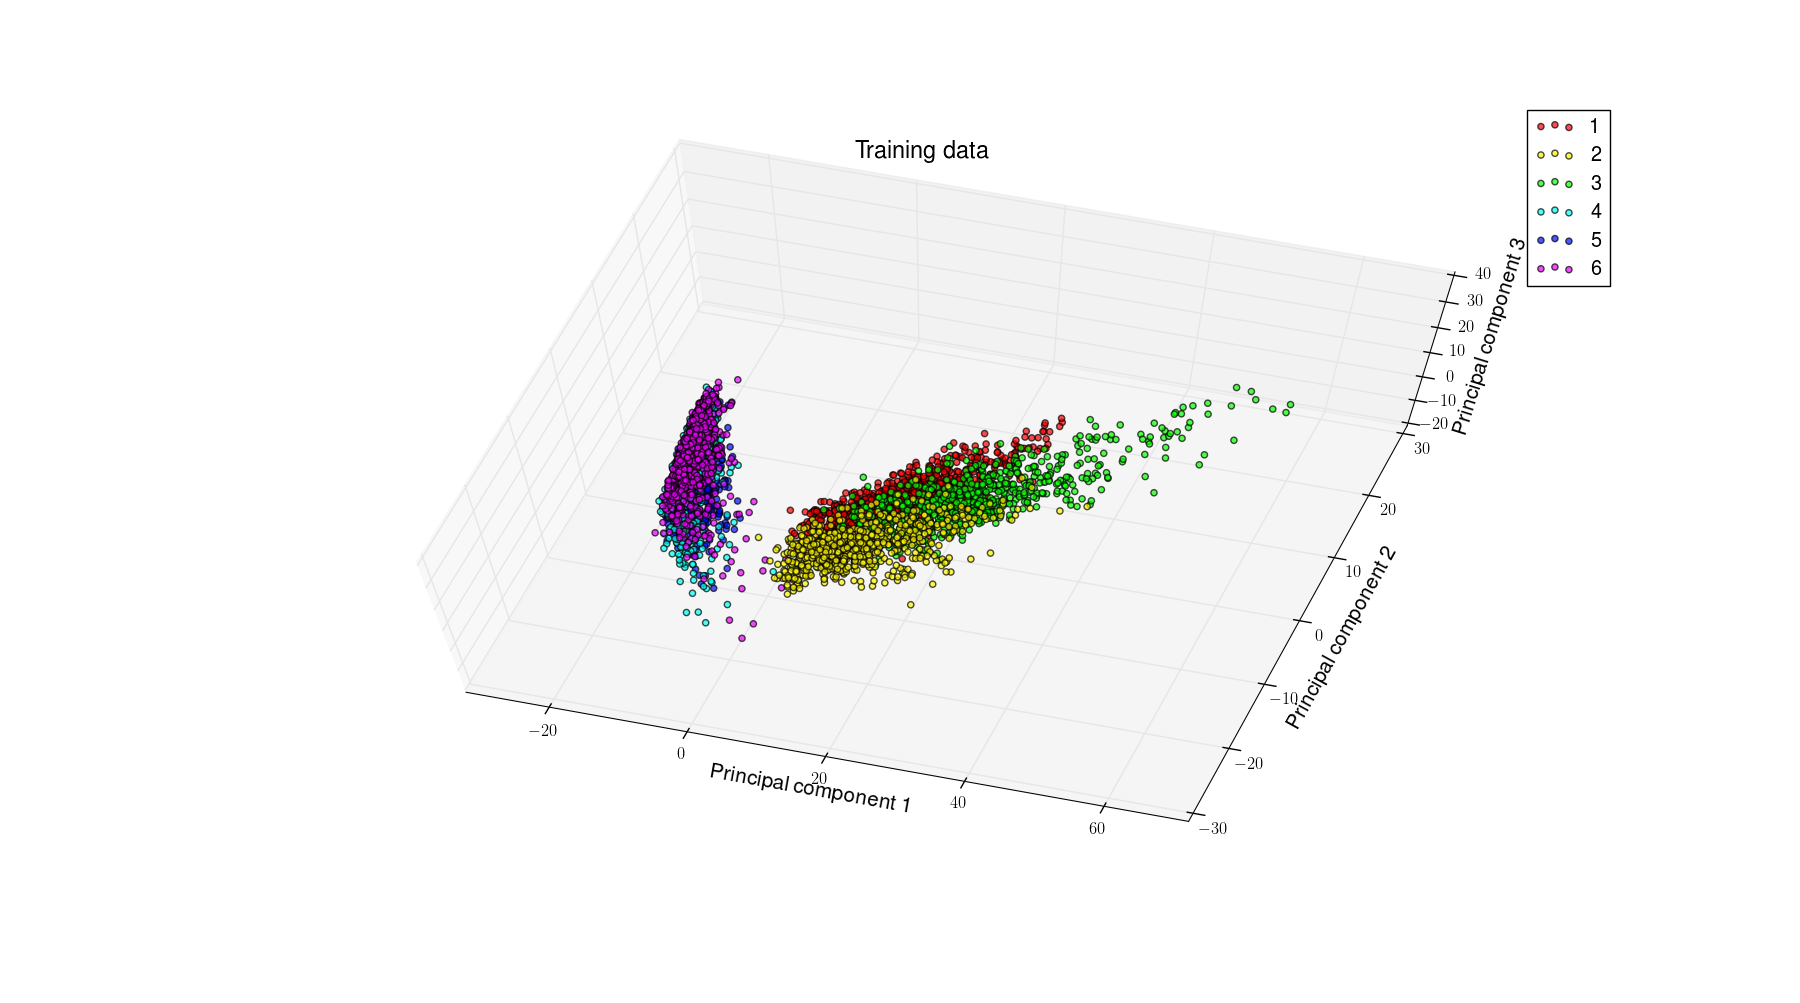
\includegraphics[scale=0.35]{Images/Xtrn.png}
		\end{center}
		\caption{Plot of the training data in the reduced space of the first three principal components}
		\label{Xtrn}
	\end{figure}
	
	\noindent
	We observe firstly that the data corresponding to the active movements seem separable from those of inactive nature. This becomes even more clear in figure \ref{Xactivity}, in which the activity type is plotted instead of the labels of the instances. The labelling of the activity types shown in figure \ref{Xactivity} will be used to distinguish the two and specify which is meant, as it is not known which of the two corresponds to the high (or low) activities. Lastly, the data corresponding to the two activity types have a clearly different shape. It therefore makes sense to plot these separately. In figures \ref{Xtrn1} and \ref{Xtrn2}, these separate plots are shown.
	
	\begin{figure}[H]
		\begin{center}
			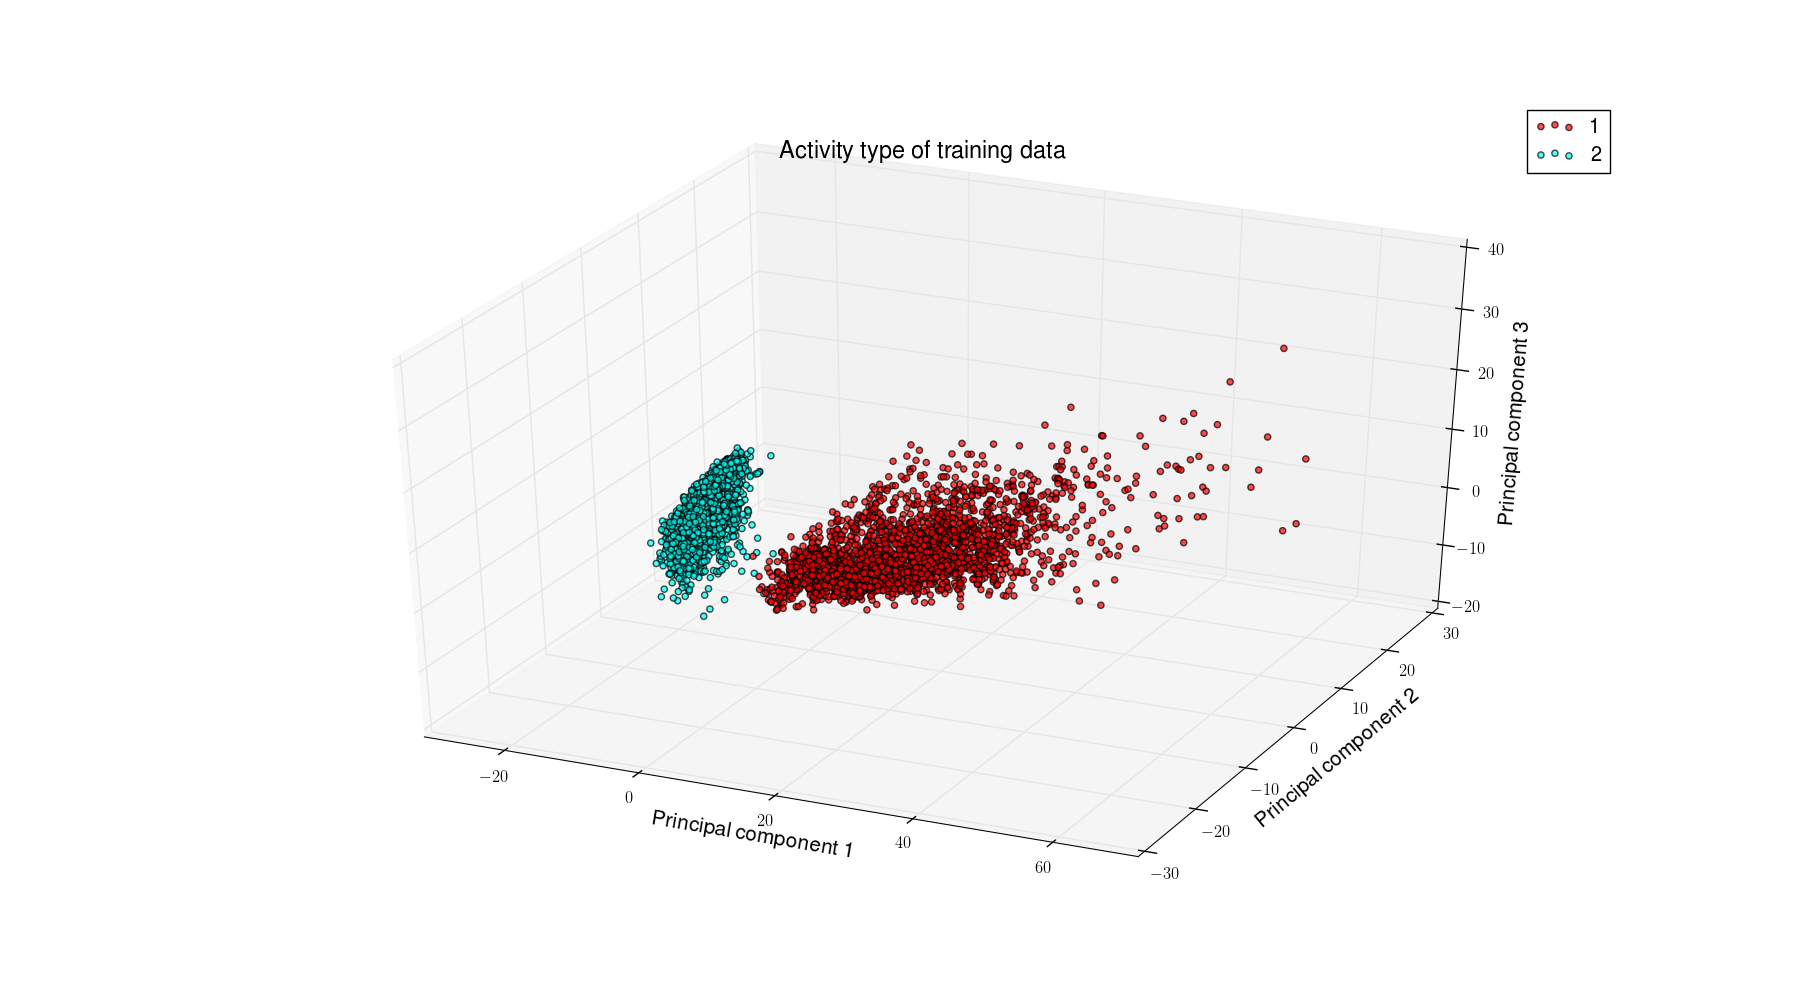
\includegraphics[scale=0.35]{Images/Xactivity.png}
			\caption{Plot of the activity types of the training data}
			\label{Xactivity}
		\end{center}
	\end{figure}
	
	\begin{figure}[H]
		\begin{center}
			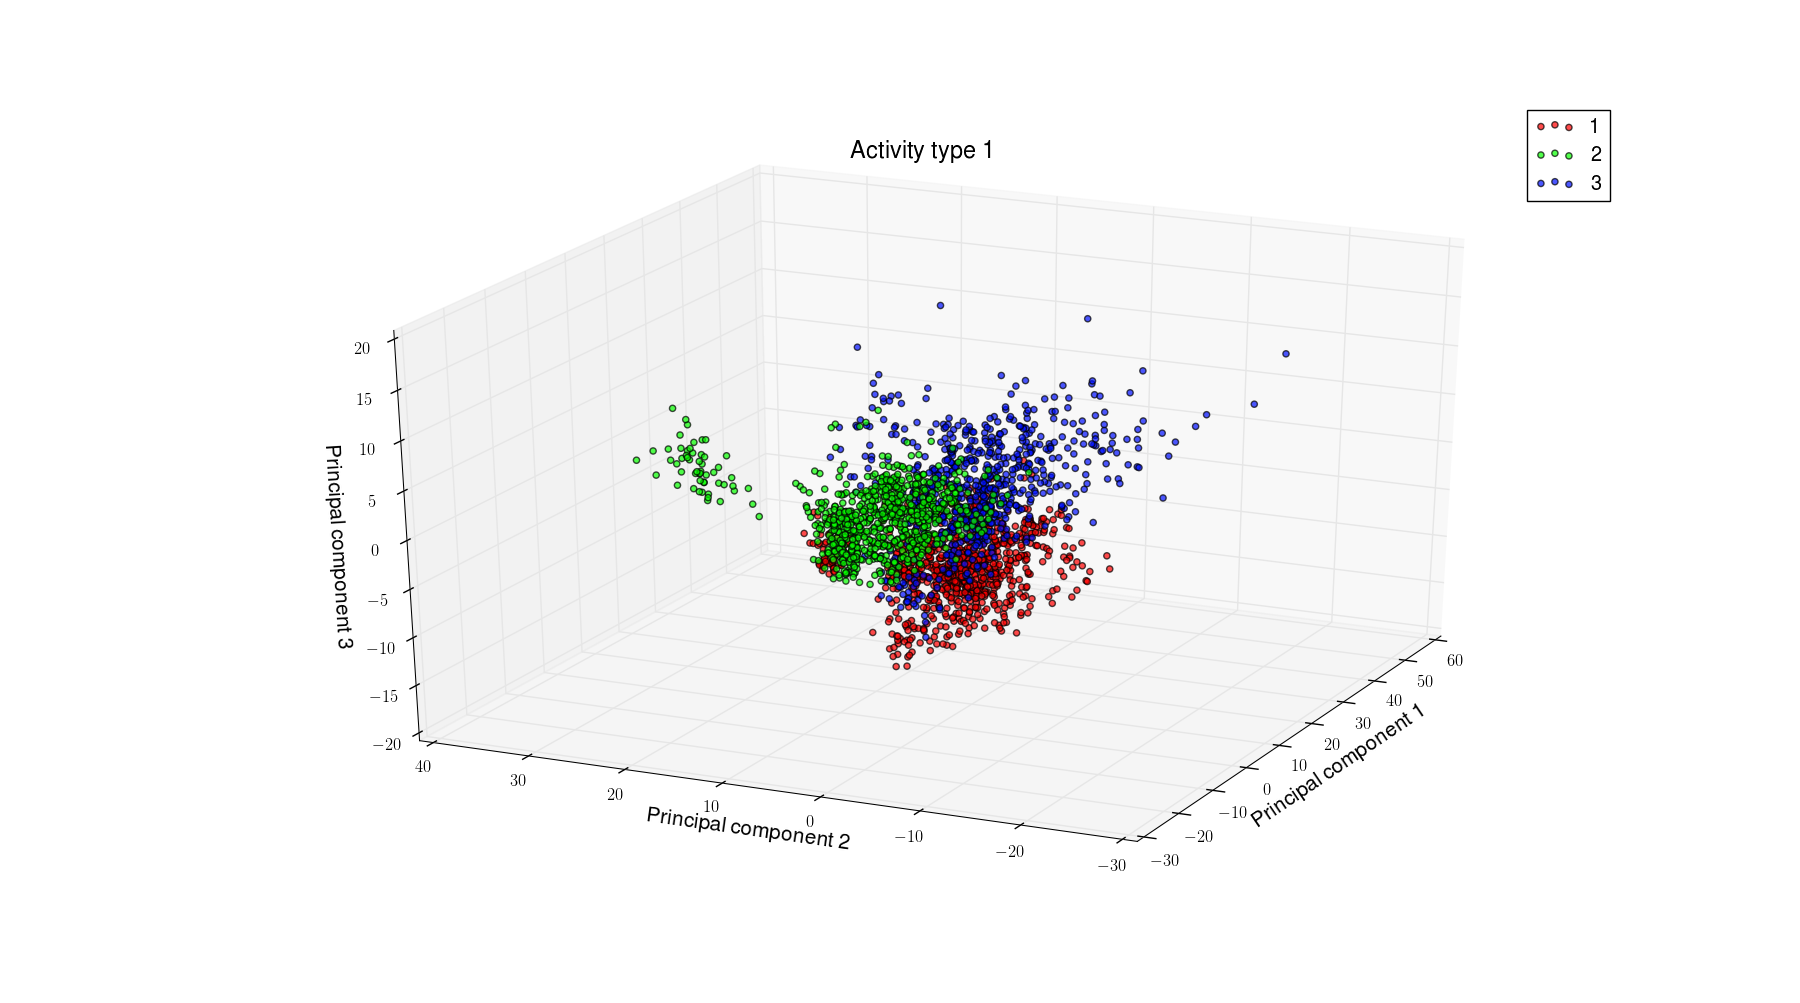
\includegraphics[scale=0.35]{Images/Xtrn1.png}
			\caption{Plot of the training data corresponding to activity type 1 in the reduced space of the first three principal components}
			\label{Xtrn1}
		\end{center}
	\end{figure}
	
	\begin{figure}[H]
		\begin{center}
			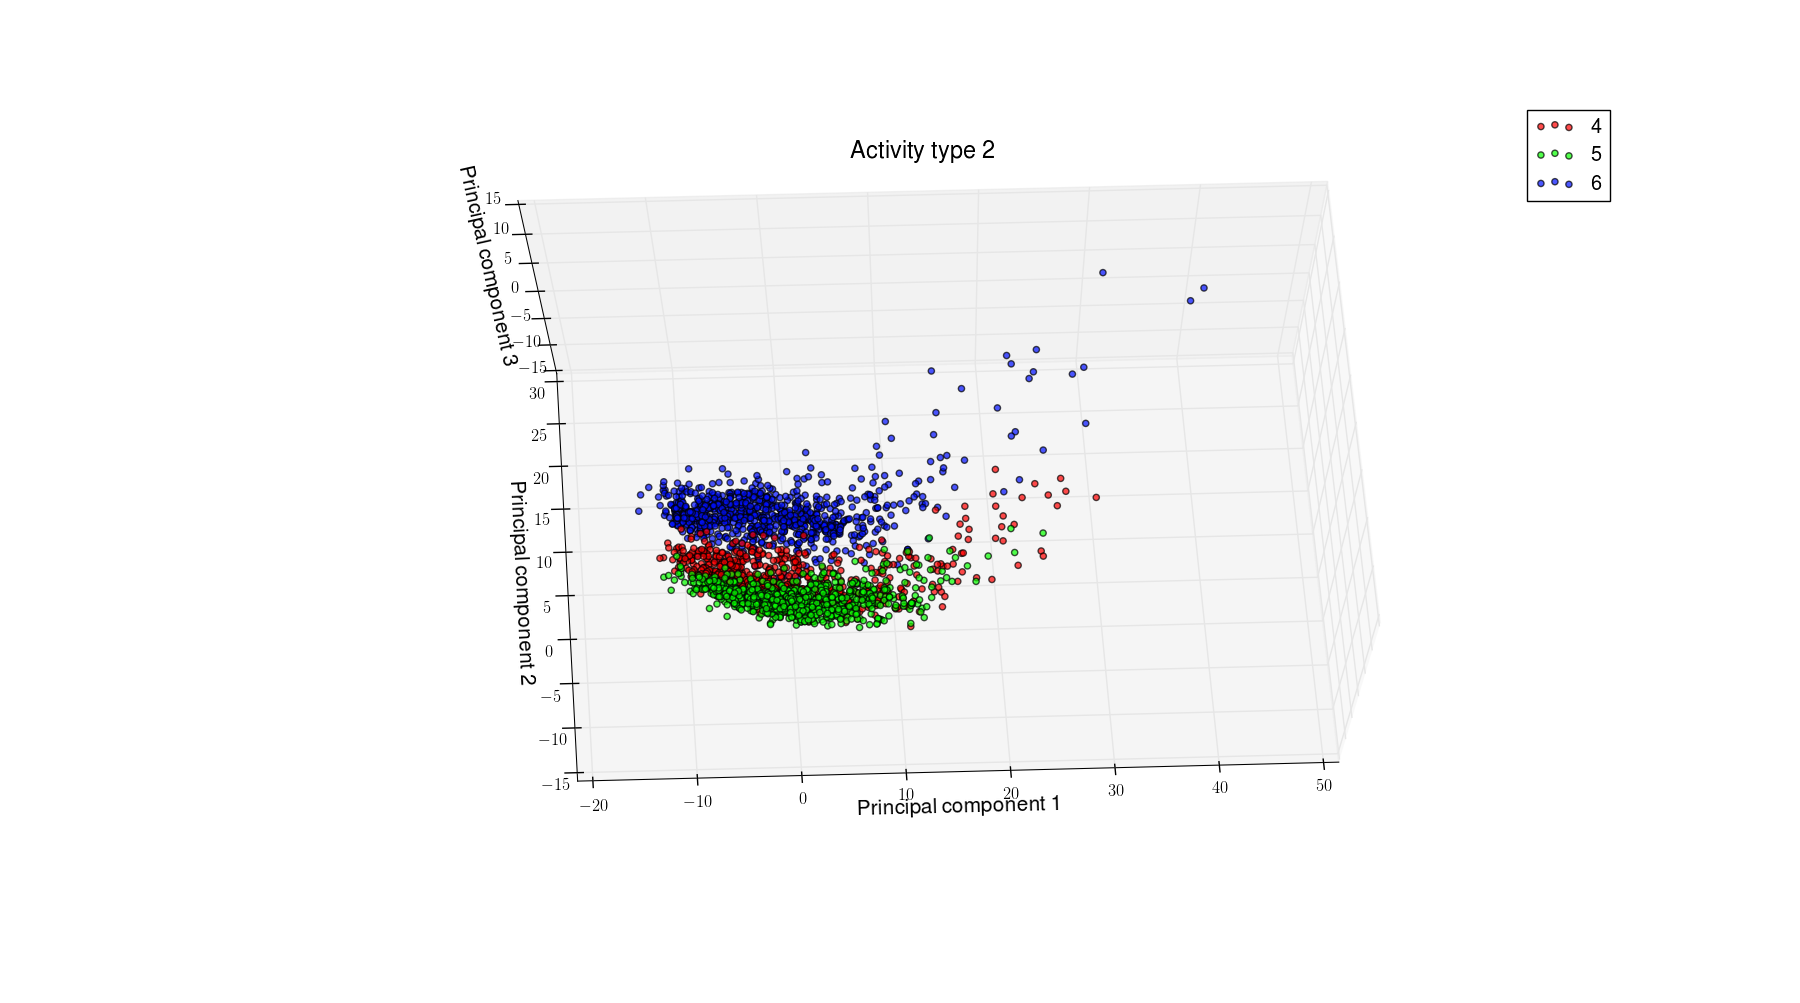
\includegraphics[scale=0.35]{Images/Xtrn2.png}
			\caption{Plot of the training data corresponding to activity type 1 in the reduced space of the first three principal components}
			\label{Xtrn2}
		\end{center}
	\end{figure}
	
	\noindent
	Based on these images, it seems that the labels corresponding to activity type 1 are not completely separable. On the other hand, the ones of activity type 2 seem separable by some non-linear manifold.\\
	
	\noindent
	As the identifiers are also given, we are enabled to look at the data coming from a single subject for both activity types. This is shown for a few subjects in figure \ref{subjects}.
	
	\begin{figure}[H]
		\begin{center}
			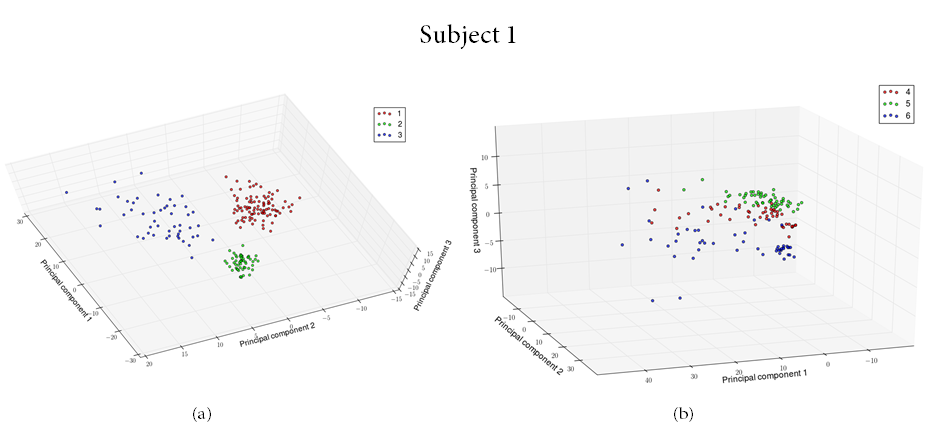
\includegraphics[scale=0.6]{Images/subject1.png}
		\end{center}

		\begin{center}
			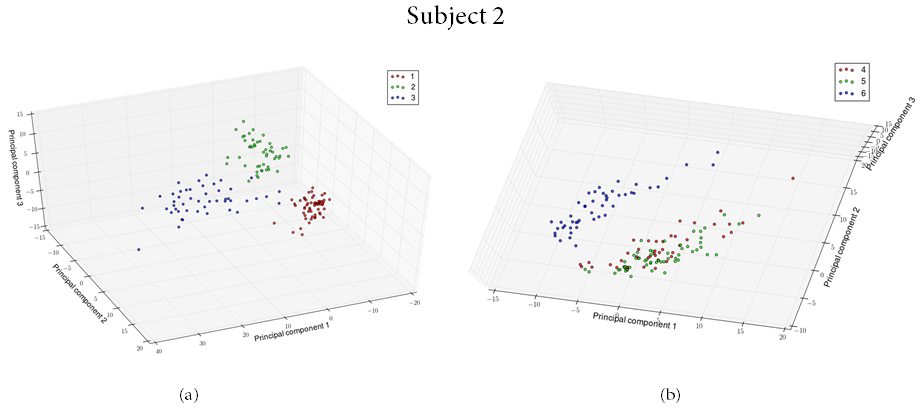
\includegraphics[scale=0.6]{Images/subject2.png}
		\end{center}

		\begin{center}
			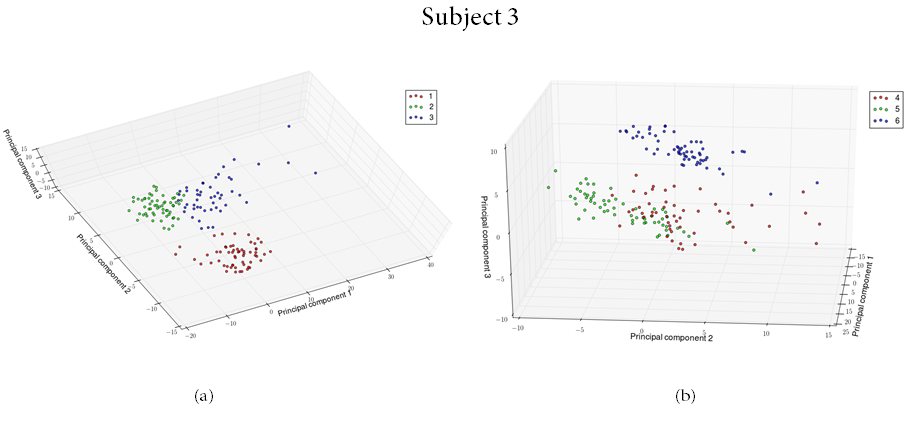
\includegraphics[scale=0.6]{Images/subject3.png}
		\end{center}
		\caption{Plot the data coming from one of the subjects. Both the instances of activity type 1 (a) and type 2 (b) are shown.}
		\label{subjects}
	\end{figure}
	
	\noindent
	Firstly, we observe that per subject, the labels of activity type 1 form (separate) clusters. Secondly, class 6 seems separable from class 4 and 5, but the latter two do not seem separable. This also corresponds with figure \ref{Xtrn2}. \\
	
	\noindent
	Finally, we plot both the training and the test set in a single plot in figure \ref{Xall}, as to verify that the training set is representative for the test set, for if this is not the case, one could not expect the classifier trained on the training set to perform well on the test set. It may be that some correction has to be applied, such as in the covariate shift setting. However, in this case it does seem that both datasets are drawn the same distribution, or at least very similar ones. 
	
	\begin{figure}[H]
		\begin{center}
			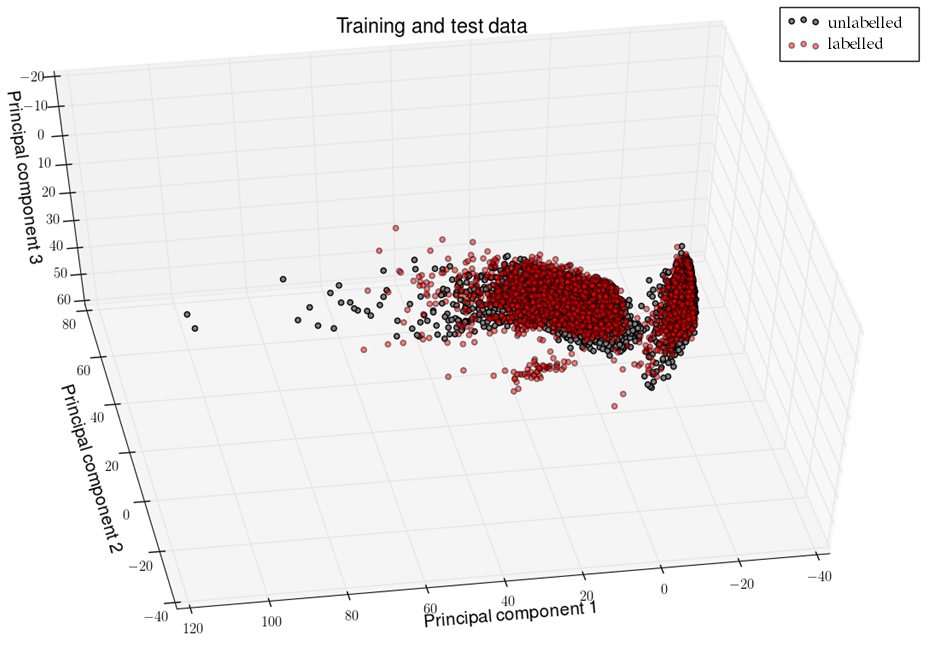
\includegraphics[scale=0.35]{Images/Xall.png}
			\caption{Plot of both the training data (labelled) and the test data (unlabelled).}
			\label{Xall}
		\end{center}
	\end{figure}
	
	
	
	\section*{Building the classifier}
	
	\subsection*{On the training data}
	
	We now start to optimize a classifier for this specific problem. We first try some basic classifiers on the training data to find out which suit the problem well and to establish some baseline on the accuracy. In table \ref{tab:basic}, the accuracy of a few classifiers on the training set is shown, evaluated using 10-fold cross-validation. For the support vector machines (SVM), a trade-off parameter of $C=10$ was used, but it was found that different values did not influence the performance that much.
	
	\begin{table}[H]
		\centering
		\caption{Accuracy of standard classifiers on the training data, evaluated using 10-fold cross-validation. A random forest classifier with $N$ estimators and criterion $A$ is denoted by RFC(N=N, criterion=$A$). The criteria 'gini', for the Gini impurity and 'entropy' for the information gain are used.}
		\label{tab:basic}
		\begin{tabular}{l|l}
			Classifier 							& Accuracy  \\ \hline
			KNN(K=3)						 	& $0.881 \pm 0.031 $\\
			KNN(K=5) 							& $0.889 \pm 0.027 $\\
			KNN(K=11) 							& $0.894 \pm 0.030 $\\
			LDA 								& $0.964 \pm 0.031 $\\
			SVC(C=10, kernel='rbf') 			& $0.950 \pm 0.036 $\\
			SVC(C=10, kernel='linear') 			& $0.951 \pm 0.032 $\\
			SVC(C=10, kernel='poly', degree=2) 	& $0.944 \pm 0.037 $\\
			SVC(C=10, kernel='poly', degree=3) 	& $0.955 \pm 0.032 $\\
			SVC(C=10, kernel='poly', degree=5) 	& $0.957 \pm 0.032 $\\
			RFC(N=100, criterion='gini')		& $0.927 \pm 0.051 $\\
			RFC(N=100, criterion='entropy')		& $0.931 \pm 0.042 $\\
		\end{tabular}		
	\end{table}
	
	\noindent
	On the full training set, the SVM with a polynomial kernel of degree 3 was able to score an accuracy of 1 on the training set. It therefore immediately becomes clear that the training data is separable, contrary to what might be expected from figure \ref{Xtrn}. This is not necessarily unexpected since the plots only show the data in reduced dimensions. Secondly, it appears that both LDA and support vector machines suit the problem very well.\\
	
	\noindent
	As the low and high activity instances appear to be separable, an idea is to first train a classifier to predict the activity type, i.e., type 1 or 2, in order to reduce the problem to two separate ones and then train different classifiers on the two sub-problems. Especially since the distributions of data from the two activity types seem to be different, one might also expect different classifiers to perform better on the two sub-problems. The obtained classifier thus uses three different classifiers. It will be denoted by $\text{SP(preClassifier, classifier1, classifier2})$ (for 'splitting classifier').
	In order to find out which classifiers work well on the two sub-problems, the training data is split based on the activity type, yielding $X_{\text{trn1}}$ and $X_{\text{trn2}}$, after which once again a 10-fold cross-validation scheme was followed to evaluate the classifiers. The result is shown in table \ref{tab:basic_separated}
	
	\begin{table}[H]
		\centering
		\caption{Accuracy of standard classifiers on the training data, evaluated using 10-fold cross-validation. A random forest classifier with $N$ estimators and criterion $A$ is denoted by RFC(N=N, criterion=$A$). The criteria 'gini', for the Gini impurity and 'entropy' for the information gain are used.}
		\label{tab:basic_separated}
		\begin{tabular}{l|l|l}
			Classifier 							& Accuracy on $X_{\text{trn1}}$ & Accuracy on $X_{\text{trn2}}$ \\ \hline
			KNN(K=3)						 	& $0.921 \pm 0.041 $			& $0.845 \pm 0.049 $\\
			KNN(K=5) 							& $0.922 \pm 0.033 $			& $0.858 \pm 0.050 $\\
			KNN(K=11) 							& $0.918 \pm 0.032 $			& $0.872 \pm 0.060 $\\
			LDA 								& $0.982 \pm 0.023 $			& $0.937 \pm 0.043 $\\
			SVC(C=10, kernel='rbf') 			& $0.962 \pm 0.041 $			& $0.942 \pm 0.040 $\\
			SVC(C=10, kernel='linear') 			& $0.968 \pm 0.028 $			& $0.937 \pm 0.043 $\\
			SVC(C=10, kernel='poly', degree=2) 	& $0.960 \pm 0.041 $			& $0.931 \pm 0.043 $\\
			SVC(C=10, kernel='poly', degree=3) 	& $0.970 \pm 0.030 $			& $0.943 \pm 0.041 $\\
			SVC(C=10, kernel='poly', degree=5) 	& $0.970 \pm 0.030 $			& $0.946 \pm 0.042 $\\
			RFC(N=100, criterion='gini')		& $0.932 \pm 0.048 $			& $0.925 \pm 0.062 $\\
			RFC(N=100, criterion='entropy')		& $0.943 \pm 0.036 $			& $0.925 \pm 0.059 $\\
		\end{tabular}		
	\end{table}
	
	\noindent
	It can be seen that classifiers generally perform better on $X_{\text{trn1}}$ than on $X_{\text{trn2}}$, indicating that the latter is less separable. Taking further into consideration figures \ref{Xtrn2} and \ref{subjects}, it seems that especially labels 4 and 5 are problematic. \\
	It also becomes clear that LDA is extremely well-fit for $X_{\text{trn1}}$. This may be explained by figure \ref{subjects}, in which it becomes apparent that the different clusters resemble Gaussian distributions. The distribution of $X_{\text{trn1}}$ is a weighted sum of the distributions of the data from the various subjects, which seem well approximated by Gaussian distributions. As a weighted sum of Gaussians is once again Gaussian, $X_{\text{trn1}}$ is expected to meet the assumptions of LDA, explaining the good performance of LDA on $X_{\text{trn1}}$. \\
	However, both LDA and a linear SVM do not perform well on $X_{\text{trn2}}$, which is readily explained by figure \ref{Xtrn2}, in which it can be seen that $X_{\text{trn2}}$ is not linearly but rather non-linearly separable. The reason behind the superior performance of the polynomial support vector machines of various degrees is therefore clear.\\
	
	\noindent
	Next, we evaluate a few classifiers to find out which separates the two sub-problems best. The result is summarized in table \ref{tab:separator}.
	
	\begin{table}[H]
		\centering
		\caption{Accuracy of standard classifiers on the activity type of the training data, evaluated using 10-fold cross-validation.}
		\label{tab:separator}
		\begin{tabular}{l|l}
			Classifier 							& Accuracy  \\ \hline
			LDA 								& $1 \pm 0 $\\
			SVC(C=10, kernel='rbf') 			& $0.9994 \pm 0.0014 $\\
			SVC(C=10, kernel='linear') 			& $0.9998 \pm 0.0006 $\\
			SVC(C=10, kernel='poly', degree=2) 	& $0.9998 \pm 0.0006 $\\
			SVC(C=10, kernel='poly', degree=3) 	& $0.9996 \pm 0.0017 $\\
			SVC(C=10, kernel='poly', degree=5) 	& $0.9996 \pm 0.0017 $\\
		\end{tabular}		
	\end{table}
	
	\noindent
	It is thus expected that using the splitting classifier in combination with LDA as both the activity-type and $X_{\text{trn1}}$ predicting classifier and a SVM with polynomial kernel of degree 5 performs best on the training data. To verify this, a few combinations are evaluated using 10-fold cross-validation. The result is shown in table \ref{tab:Xtrn_final}, which is as expected. 
	
	\begin{table}[H]
		\centering
		\caption{Accuracy of the splitting classifier in combination with various classifiers, evaluated using 10-fold cross-validation.}
		\label{tab:Xtrn_final}
		\begin{tabular}{l|l|l|l}
			Pre-classifier 					& Classifier1 					&  Classsifier2								& Accuracy  \\ \hline
			LDA 							& LDA							& SVC(kernel='rbf')) 						& $0.962 \pm 0.03 $\\
			LDA 							& LDA							& SVC(kernel='poly', degree=3)) 			& $0.962 \pm 0.03 $\\
			LDA 							& LDA							& SVC(kernel='poly', degree=5)) 			& $0.964 \pm 0.03 $\\
			LDA 							& SVC(kernel='poly', degree=3)	& SVC(kernel='poly', degree=5)) 			& $0.958 \pm 0.03 $\\
			SVC(kernel='poly', degree=2) 	& LDA							& SVC(kernel='poly', degree=5)) 			& $0.964 \pm 0.03 $\\
		\end{tabular}		
	\end{table}
	
	
	\subsection*{On the test data}
	After having evaluated some classifiers on the training data, we continue to optimize the classifier on the test data. \\
	From now on, let:
	\begin{align*}
		\text{CL A} &:= \text{SP(SVC(kernel='poly', degree=2), LDA, SVC(kernel='poly', degree=3))}\\
		\text{CL B} &:= \text{SP(SVC(kernel='poly', degree=2), LDA, SVC(kernel='poly', degree=5))}\\
		\text{CL C} &:= \text{SP(LDA, LDA, SVC(kernel='poly', degree=5))}\\
	\end{align*}
	A basic SVM with polynomial kernel of degree 3 yields a score of 0.94588 and and $\text{CL A}$ scores 0.96774. It is thus verified that the classifiers generalize well on the test-data and achieve quite a high accuracy. \\
	
	\noindent
	The identifiers can potentially be used to boost the performance of the classifier. This is attempted by varying the weight of the instances based on the variance of the data $X_{s,l}$ with some label $l$ belonging to a certain subject $s$. The idea is that a larger variance corresponds to more uncertainty, so that these instances are given a lower weight. The weight is determined by first fitting a Gaussian distribution on $X_{s,l}$ for each subject and each label, yielding a covariance matrix $\Sigma$. We next define $\sigma_{s,l} = tr(\Sigma)$, where $tr(.)$ stands for the trace of a matrix. Thus, $\sigma_{s,l}$ represents the total variance of $X_{s,l}$. Finally, we define the weights of the instances in $X_{s,l}$ to be:
	$$ w_{s,l} = { \sum_{s\in\mathcal{S}}\sigma_{s,l} \over \sigma_{s,l} } $$
	Where $\mathcal{S}$ is the set of all subjects. Using these weights barely improves the performance on the training set of a SVM with polynomial kernel of degree 2 from $0.947 \pm 0.032$ to $0.0948 \pm 0.033$. On each of the classifiers $\text{CL A/B/C}$, it has no effect.\\
	
	\noindent
	As the problem is of transductive/semi-supervised nature, the test data can be used in the training process to increase the performance, to which there are multiple approaches. As many of the test instances were be predicted with high confidence, self-learning  seems very promising. A label-propagation approach was also considered, but after training on the full dataset, this yielded a poor score on the training data and was thus discarded. The self-learning is implemented in a manner in which test instances are added to the labelled data if they are predicted with a confidence higher than a certain threshold. This threshold decreases per iteration, from 0.99 to 0.6 in 200 iterations. Furthermore, test instances that are added to the labelled data during the $i^{th}$ iteration are given a weight of $\gamma^{i}$ for some $\gamma \in (0,1]$, taking into account that labels that are predicted during a later stage have a higher uncertainty, both due to the unstable nature of self-learning (an error early may grow in further iterations), and the lower threshold in a later iteration, and should thus receive a lower weight. This is a parameter that can be tuned based on the desired behaviour of the self-learner.\\
		
	\noindent
	The performance on $X_{\text{trn}}$ of various of the best performing self-learning classifiers is summarized in table \ref{tab:Xst_selfLearning}.
	
	\begin{table}[H]
		\centering
		\caption{Score of self-learning classifiers on the test set $X_{\text{trn}}$. The self-learner is combined with various classifiers.}
		\label{tab:Xst_selfLearning}
		\begin{tabular}{ll|l}
			Classifier 		& $\gamma$ 	& Score  		\\ \hline
			$\text{CL A}$ 	& 1			& $0.97724$		\\
			$\text{CL A}$ 	& 0.99		& $0.97545$		\\
			$\text{CL B}$ 	& 1			& $0.97760$		\\
			$\text{CL B}$ 	& 0.995		& $0.97724$		\\
			$\text{CL B}$ 	& 0.99		& $0.97742$		\\
			$\text{CL C}$ 	& 0.998		& $0.97814$		\\
		\end{tabular}		
	\end{table}
	
	\noindent
	We thus conclude that the self-learning algorithm did indeed improve the performance considerably. Furthermore, we find that the self-learner combined with $\text{CL C}$ has the best score, as expected.  
	
	\section*{Final thoughts}
	It was concluded that the self-learning algorithm combined with $\text{CL C}$ has the best performance with a score of $0.97814$. \\\\
	By somehow making use of the identifiers, it may be possible to achieve an even higher score. Usually in machine learning problems, the instances are assumed to be independent and identically distributed. However, this is not the case as instances stemming from the same subject are clearly not independent, which may lower performance of certain classifiers. It might be possible to use the identifiers to deal with this problem, thus potentially increasing the score. \\\\
	Secondly, multiple well-performing algorithms can be combined in either some majority voting or confidence based scheme, potentially improving the final score. However, in this case the various well-performing predictions are very similar so that a large boost can not be expected. In fact, this was attempted by combining all but the self-learning algorithm combined with the $\text{CL C}$ classifier, which had not been submitted yet, but it resulted in the same score as the best of the classifiers in the ensemble.\\\\
	One more suggestion might be to use a transductive algorithm such as a the transductive support vector machine(T-SVM) and possibly to combine such algorithms somehow with the self-learning $\text{CL C}$ classifier obtained in this report. Since the problem is in a transductive setting, such an algorithm may be beneficial. However, as no easily accessible implementation was found and it was assumed that the self-learning algorithm in this case is superior, it was decided not to try and implement the T-SVM.\\\\
	Lastly, one could continue fine-tuning parameters or improving certain parts of the final classifier, which may improve the score.
	
	
\end{document}